\documentclass[a4paper,10pt]{report}
\usepackage[utf8]{inputenc}
\usepackage{amsmath}
\usepackage{graphicx, listings, hyperref}
\lstloadlanguages{Ruby}

% Title Page
\title{Approximation du nombre $$\pi$$}
\author{Nicolas Iung, Aurélien Blais}

\begin{document}
\maketitle

\chapter{Méthode des séries}
\section{Somme des inverses des carrés}

\subsection{Question 1}
\subsubsection{Montrer que $a_0$ = 0}
On sait d'après l'énoncé que sur l'intervalle $]0, \pi[$, $f(t) = 1$ et que sur l'intervalle $]-\pi, 0[$, $f(t) = -1$\\

\begin{align*}
a_0 &= \frac{1}{2\pi} \int_{0}^{2\pi} f(t)dt \\
a_0 &= \frac{1}{2\pi} (\int_{0}^{\pi} 1 dt + \int_{\pi}^{2\pi} -1 dt)\\
a_0 &= \frac{1}{2\pi} (\pi - \pi)\\
a_0 &= 0
\end{align*}

\subsubsection{Montrer que $a_n$ = 0}
\begin{align*}
a_n &= \frac{2}{2\pi} \int_{0}^{2\pi} f(t)cos(nt) dt \\
a_n &= \frac{2}{2\pi} (\int_{0}^{\pi} cos(nt) dt + \int_{\pi}^{2\pi} -cos(nt) dt)\\
a_n &= \frac{2}{2\pi} (\frac{sin(n\pi)}{n} - \frac{sin(n\pi)}{n} )\\
a_n &= 0
\end{align*}

\subsubsection{Montrer que $b_n = \frac{4}{2\pi}(\frac{1-cos(n\pi)}{n})$}
\begin{align*}
b_n &= \frac{2}{2\pi} \int_{0}^{2\pi} f(t) sin(nt) dt\\
b_n &= \frac{2}{2\pi} (\int_{0}^{\pi} sin(nt) dt + \int_{\pi}^{2\pi} -sin(nt) dt)\\
b_n &= \frac{2}{2\pi} [(\frac{1}{n} - \frac{cos(n\pi)}{n}) + \frac{cos(2n\pi) - cos(n\pi)}{n}]\\
b_n &= \frac{2}{2\pi} [\frac{1}{n} (-cos(n\pi) + 1 + cos(2n\pi) - cos(n\pi))]\\
b_n &= \frac{2}{2\pi} [\frac{1}{n} (-2cos(n\pi) + 2)]\\
b_n &= \frac{2}{2\pi} [\frac{2}{n} (-cos(n\pi) + 1)]\\
b_n &= \frac{4}{2\pi} [\frac{1 - cos(n\pi)}{n}]
\end{align*}

\subsection{Question 2}
Etudions $b_n$ lorsque n est pair ou impaire.
Cela reviens a calculer $b_n$ pour $2p$ et $2p+1$

\subsubsection{Calculons $b_{2p}$}
\begin{equation*}
b_{2p} = \frac{4}{2\pi}*\frac{1-cos(2p\pi)}{2p}\\
\end{equation*}
Or $\forall x  	\in R, cos(2p\pi) \Leftrightarrow  cos(2\pi) = 1$
\begin{align*}
b_{2p} &= \frac{4}{2\pi}*\frac{1-1}{2p}\\
b_{2p} &= \frac{4}{2\pi}*\frac{0}{2p}\\
b_{2p} &= \frac{4}{2\pi}*0\\
b_{2p} &= 0
\end{align*}

\subsubsection{Calculons $b_{2p+1}$}
\begin{align*}
b_{2p+1} &= \frac{4}{2\pi}(\frac{1-cos((2p+1)\pi)}{2p+1})\\
b_{2p+1} &= \frac{4}{2\pi}(\frac{1-cos(2p\pi+\pi)}{2p+1})\\
b_{2p+1} &= \frac{4}{2\pi}(\frac{1-cos(\pi)}{2p+1})\\
b_{2p+1} &= \frac{4}{2\pi}(\frac{1-(-1)}{2p+1})\\
b_{2p+1} &= \frac{4}{(2p+1)\pi}\\
\end{align*}

\subsection{Question 3}
\subsubsection{Montrer que, pour f, $\sum_{p=0}^{+\infty} = \frac{1}{(2p + 1)^2} = \frac{\pi^2}{8}$}
\begin{align*}
A &= \frac{1}{2\pi}\int_{0}^{2\pi} |f(t)|^2 dt = |a_0|^2 + \frac{1}{2}(\sum_{n=1}^{+\infty} |a_n|^2 + |b_n|^2)\\
A &= \frac{1}{2}(\sum_{n=1}^{+\infty} |\frac{2}{2\pi} \int_{0}^{2\pi} f(t)cos(nt)dt)|^2 + |\frac{2}{2\pi}\int_{0}^{2\pi}f(t)sin(nt)|^2)\\
A &= \frac{1}{2}(\sum_{n=1}^{+\infty} |\frac{2}{2\pi} \int_{0}^{2\pi} f(t)sin(nt)dt)|^2)\\
A &= \frac{1}{2}(\sum_{n=1}^{+\infty} |\frac{4}{2\pi}[\frac{1-cos(n\pi)}{n}]|^2)\\
A &= \frac{1}{2}(\sum_{p=0}^{+\infty} |\frac{4}{2\pi}[\frac{1-cos((2p+1)\pi)}{2p+1}]|^2 + \sum_{p=1}^{+\infty} |\frac{4}{2\pi}[\frac{1-cos(2p\pi)}{2p}]|^2)\\
A &= \frac{1}{2}(\sum_{p=0}^{+\infty} |\frac{4}{2\pi}[\frac{1-cos((2p+1)\pi)}{2p+1}]|^2)\\
A &= \frac{1}{2}(\sum_{p=0}^{+\infty} |\frac{4}{(2p+1)\pi}|^2)\\
A &= \frac{8}{\pi^2}(\sum_{p=0}^{+\infty} (\frac{1}{2p+1})^2)\\
\text{Or } &\forall t \in [0;2\pi]; |f(t)|^2 = 1 \text{ donc}\\
A &= \frac{1}{2\pi}\int_{0}^{2\pi} |f(t)|^2 dt\\
A &= \frac{1}{2\pi}\int_{0}^{2\pi} |1|^2 dt\\
A &= \frac{1}{2\pi}[1]_0^{2\pi}\\
A &= \frac{1}{2\pi}2\pi = 1\\
A &= \frac{8}{\pi^2}\sum_{p=0}^{+\infty}(\frac{1}{2p+1})^2
\end{align*}

\subsection{Question 4}
\subsubsection{Montrer que $\sum_{n=1}^{+\infty}\frac{1}{n^2} = \frac{1}{4}\sum_{n=1}^{+\infty}\frac{1}{n^2} + \frac{\pi^2}{8}$}
\begin{align*}
\sum_{n=1}^{2N}\frac{1}{n^2} &= \sum_{p=1}^{N}\frac{1}{(2p)^2} + \sum_{p=0}^{N-1}\frac{1}{(2p+1)^2}\\
\lim_{n\to\infty} \sum_{n=1}^{2N}\frac{1}{n^2} &= \lim_{n\to\infty}(\sum_{p=1}^{N}\frac{1}{(2p)^2} + \sum_{p=0}^{N-1}\frac{1}{(2p+1)^2})\\
\sum_{n=1}^{+\infty}\frac{1}{n^2} &= \sum_{p=1}^{+\infty}\frac{1}{(2p)^2} + \sum_{p=0}^{+\infty}\frac{1}{(2p+1)^2}\\
=\sum_{p=1}^{+\infty}\frac{1}{2^2 p^2} &= \sum_{p=1}^{+\infty}\frac{1}{2^2 p^2} + \frac{\pi^2}{8}\\
=\frac{1}{4}\sum_{p=1}^{+\infty}\frac{1}{p^2} + \frac{\pi^2}{8} &= \frac{1}{4}\sum_{n=1}^{+\infty}\frac{1}{n^2} + \frac{\pi^2}{8}
\end{align*}

\subsection{Question 5}
\subsubsection{Déduire que $\sum_{n=1}^{+\infty} \frac{1}{n^2} = \frac{\pi^2}{6}$}
\begin{align*}
\text{On pose } X = \sum_{n=1}^{+\infty} \frac{1}{n^2}
\end{align*}
D'après la question précédente
\begin{align*}
X &= \frac{1}{4}X + \frac{\pi^2}{8}\\
\frac{3}{4}X &= \frac{\pi^2}{8}\\
X &= \frac{4}{3} \frac{\pi^2}{8} = \frac{\pi^2}{6}\\
\text{Donc}\\
\sum_{n=1}^{+\infty} \frac{1}{n^2} &= \frac{\pi^2}{6}
\end{align*}

\clearpage
\section{Implémentations}
\subsection{Question 1}
\subsubsection{Implémentation de \textit{SerieInvCarres(N)}}
\begin{lstlisting}[language=Ruby]
  def self.serie_inv_carres(n)
    (1..n).inject(0.0) { |sum, n| sum + 1 / (n ** 2).to_f }
  end
\end{lstlisting}
La méthode retourne la valeur de la somme de 1 à n, avec pour valeur initiale 0.0
\bigskip

\subsection{Question 2}
\subsubsection{Implémentation de \textit{MethodeSerieInvCarres(N)}}
\begin{lstlisting}[language=Ruby]
  def self.methode_serie_inv_carres(n)
    Math.sqrt(serie_inv_carres(n) * 6)
  end
\end{lstlisting}
La méthode retourne la racine carrée de la somme produite par la méthode précédente fois six
\bigskip

\subsection{Question 3}
\subsubsection{Implémentation de \textit{SerieInvCarresImparis(N)}}
\begin{lstlisting}[language=Ruby]
  def self.serie_inv_carres_imparis(n)
    return 1 / ((2 * n + 1) ** 2) if n.zero?

    n.times.inject(0.0) { |sum, n| sum + 1 / ((2 * n + 1) ** 2).to_f }
  end
\end{lstlisting}
Dans le cas où n = 0, la méthode retourne 0. Sinon de la même manière que précédemment, elle effectue la somme de 0 à n.
\bigskip

\subsection{Question 4}
\subsubsection{Implémentation de \textit{MethodeSerieInvCarresImparis(N)}}
\begin{lstlisting}[language=Ruby]
  def self.methode_serie_inv_carres_imparis(n)
    Math.sqrt(serie_inv_carres_imparis(n) * 8)
  end
\end{lstlisting}
La méthode retourne la racine carrée de la somme produit par la méthode précédente fois 8
\bigskip

\subsection{Question 5}
\subsubsection{Evolution des deux méthodes}
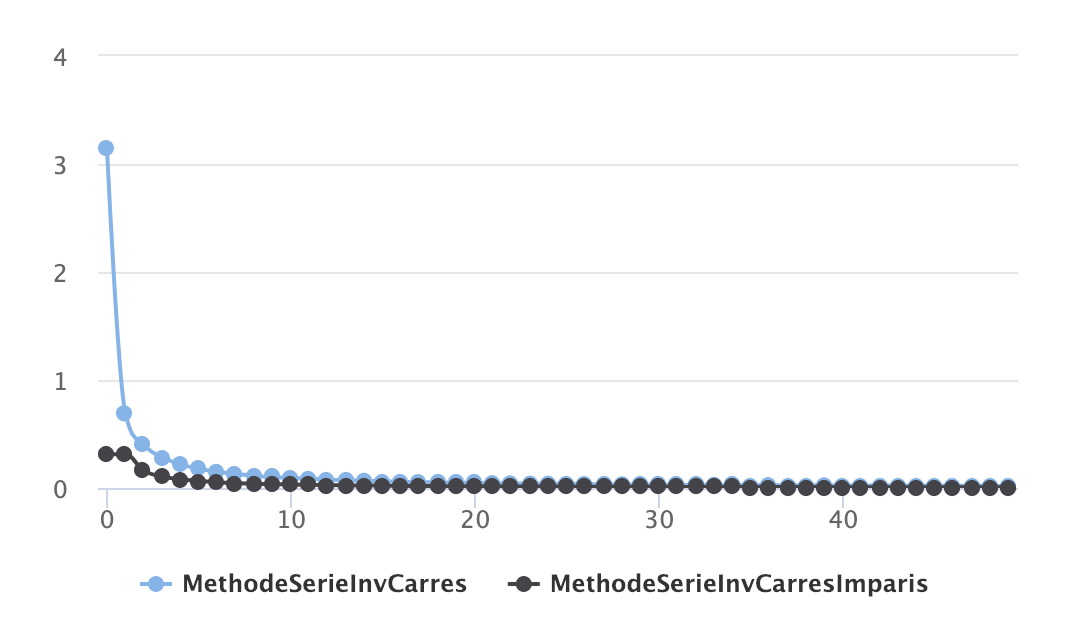
\includegraphics[scale=0.75]{images/question_5.png}
\bigskip

\subsection{Question 6}
\subsubsection{Convergence des deux méthodes}
Pour la méthode \textit{MethodeSerieInvCarres(N)}, nous avons observer une précision de l'ordre de $10^{-4}$ au terme N = 22388\\
Pour la méthode \textit{MethodeSerieInvCarresImparis(N)}, nous avons observer une précision de l'ordre de $10^{-4}$ au terme N = 7463
\bigskip

\clearpage
\subsection{Question 7}
\subsubsection{Implémentation de \textit{MethodeSerieRamanujan(N)}}
\begin{lstlisting}[language=Ruby]
  def self.methode_serie_ramanujan(n)
    1 / n.times.inject(0.0) do |sum, i|
      sum + (2 * Math.sqrt(2) / 9801).to_f * (((factorial(4 * i).to_f * (1103 + 26390 * i).to_f)).to_f / ((factorial(i).to_f ** 4) * (4 * 99) ** (4 * i).to_f).to_f)
    end
  end
\end{lstlisting}
La méthode retourne la valeur donnée par la formule énoncée dans le sujet.\\
Nous avons par ailleurs dû implémenter une méthode \textit{factorial(N)}, celle-ci n'étant pas présente nativement en Ruby, qui multiple les valeurs de 1 à N\\
\begin{lstlisting}[language=Ruby]
  def self.factorial(n)
    (1..n).reduce(1, :*)
  end
\end{lstlisting}

\subsection{Question 8}
\subsubsection{Convergence de la méthode de Ramanujan}
\begin{tabular}{|l|c|r|} 
	\hline
	n & Résultat & Nombre de chiffres exactes\\
  	\hline
	1 & 3.1415927300133055233288815 & 7\\
	\hline
	2 & 3.1415926535897935600871733 & 16\\
	\hline
	3 & 3.1415926535897931159979635 & 41\\
	\hline
	4 & 3.1415926535897931159979635 & 41\\
	\hline
	5 & 3.1415926535897931159979635 & 41\\	
	\hline	
\end{tabular}\\
La valeur de référence utilisée est donnée par la constante Ruby \textit{Math::PI}, on remarque que la méthode converge rapidement, le nombre de chiffres exactes prend en compte la partie entière du résultat.\\
A partir de la 3ème itération, la valeur reste bloquée à 41, qui est la taille maximale d'un \textit{Float} en Ruby.
\bigskip

\subsection{Question 9}
\subsubsection{Avantages et Inconvénients}
Les deux premières méthodes convergent lentement vers Pi, tandis que la méthode Ramanujan converge très rapidement.\\
Celle de Ramanujan faisant appel à des factorielles a un coût en ressources plus élevé que les deux autres.

\chapter{Méthode de Monte-Carlo}
\subsection{Question 1}
\subsubsection{Aire du disque et valeur de $\lim_{n\to\infty} \frac{k_n}{n}$}
L'aire d'un disque est obtenu par la formule $\pi R^2$, la portion ici observée a pour aire $\frac{1}{4}\pi$.\\
La valeur de $\lim_{n\to\infty} \frac{k_n}{n}$ doit tendre vers $\frac{1}{4}\pi$.
\bigskip

\subsection{Question 2}
\subsubsection{Implémentation de \textit{Tirage(N)}}
\begin{lstlisting}[language=Ruby]
  def self.tirage(n)
    Array.new(n) { [rand, rand] }
  end
\end{lstlisting}
La méthode retourne un tableau de couples ayant une valeur comprise entre $[0,1]$
\bigskip

\subsection{Question 3}
\subsubsection{Représentation du tirage}
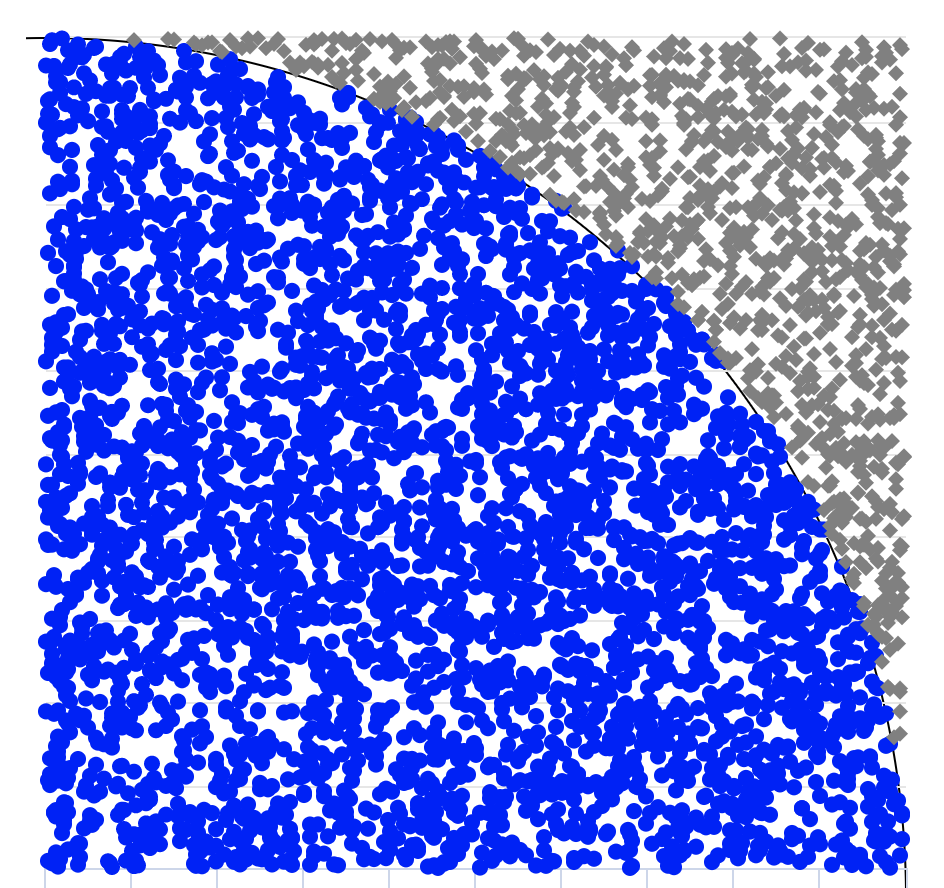
\includegraphics[scale=0.75]{images/question_2.png}
\bigskip

\clearpage
\subsection{Question 4}
\subsubsection{Implémentation de \textit{MonteCarlo(N)}}
\begin{lstlisting}[language=Ruby]
  def self.montecarlo(n)
    return 0 if n.zero?
    counter = 0
    tirage(n).each do |n|
      counter += 1 if (n[0]**2) + (n[1]**2) <= 1
    end
    counter * 4.0 / n
  end
\end{lstlisting}
La méthode retourne 0 si N = 0.\\
Sinon on incrémente un compteur pour chaque point faisant parti du cercle, en utilisant la formule donnée dans le sujet $x^2 + y^2 \leq 1$.\\
On retourne la valeur donnée en suivant la formule $\frac{k_{n}}{n}$ où $k_{n}$ est représenté par le compteur.\\
La valeur est multiplié par 4 pour obtenir une approximation de $\pi$ et non de $\frac{\pi}{4}$.
\bigskip

\subsection{Question 5}
\subsubsection{Convergence de la méthode de Monte-Carlo}
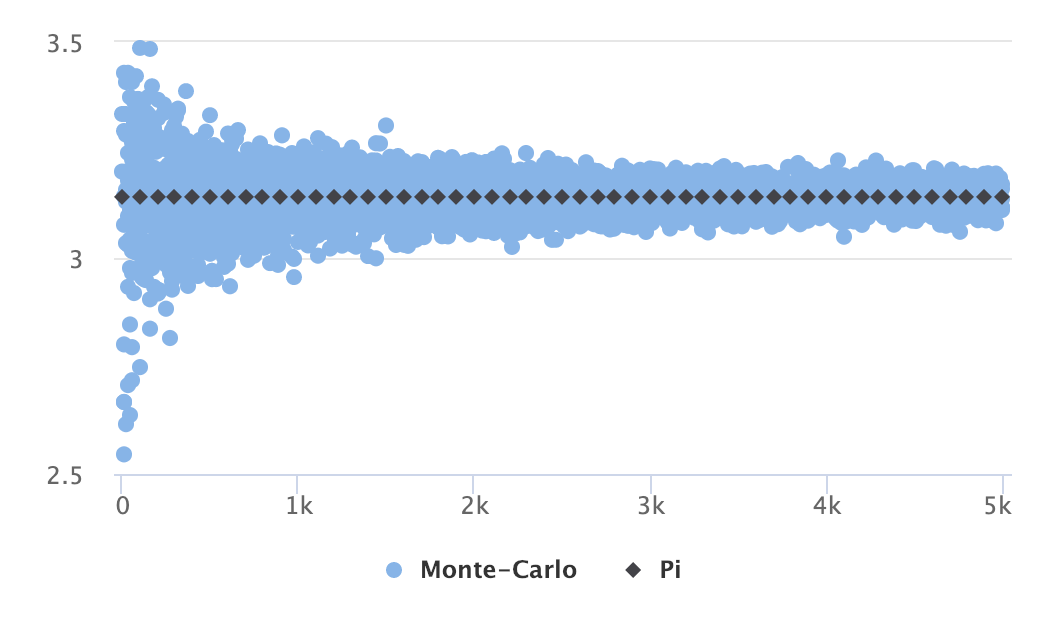
\includegraphics[scale=0.75]{images/question_2_5.png}
Les points en bleu représentent les valeurs obtenues par la méthode \textit{MonteCarlo(N)}, les points en noir représentent la valeur de \textit{Math::PI}.\\
On peut observer que la méthode semble converger vers $\pi$, cette convergence est cependant très lente et la valeur reste imprécise.\\
\bigskip

\subsection{Question 6}
\subsubsection{Convergence de la méthode de Monte-Carlo}
\begin{tabular}{|l|c|r|} 
	\hline
	Echantillon & Nombre d'itérations\\
  	\hline
	10 & 1 626\\
	\hline
	50 & 1 433\\
	\hline
	100 & 1 286\\
	\hline	
\end{tabular}\\
Pour obtenir une précision de l'ordre de $10^{-4}$, en répétant l'expérience 100 fois, nous observons une moyenne de 1286 points.
\bigskip

\subsection{Question 7}
\subsubsection{Comparaison avec les méthodes des séries}
Cette méthode ne converge que très lentement et nécessite un nombre d'itérations important pour obtenir une valeur imprécise.

\chapter{Ouverture}
\subsection{Question 1}
\subsubsection{Méthode de calcul différente}
On peut citer la méthode d'Archimèdes.\\
Le principe étant que nous savons calculer le périmètre d'un polygone. Il utilise donc deux polygones à 6 côté, l'un inscrit et l'autre conscrit à un cercle de rayon $\frac{1}{2}$.\\
En augmentant le nombre de côtés des polygones, ceux-ci commenceront à se confondre avec le cercle, et il devient alors possible d'approximer $\pi$\\

\bigskip
Exemple d'implémentation algorithmique en Ruby
\begin{lstlisting}[language=Ruby]
def self.archimedes(n)
  v = 4.0
  u = 2.0 * Math.sqrt(2.0)
  mean = (u+v) / 2.0

  (1..n).each do |i|
    v = v*u/mean
    u = Math.sqrt(v*u)
    mean = (u+v)/2
  end
  mean
end

ruby2.5.3 > archimedes(1)
 => 3.18758797895274
ruby2.5.3 > archimedes(10)
 => 3.1415928075997126
ruby2.5.3 > archimedes(100)
 => 3.1415926535897927
\end{lstlisting}
\textit{u} étant la longueur d'un côté du polygone inscrit et \textit{v} la longueur d'un côté du polygone circonscrit.

\subsection{Question 2}
\subsubsection{Modélisation en Ruby}
En Ruby, la valeur de $\pi$ la valeur est codée en dur lors de la compilation de l'interpréteur, écrit en C.
\begin{lstlisting}[language=C]
#ifndef M_PI
# define M_PI 3.14159265358979323846
#endif
\end{lstlisting}
Cette valeur étant limitée à 20 décimales (la taille d'un \textit{double} en C), s'il y a besoin d'une plus grande précision, l'interpréteur utilise la formule de Ramanujan pour la calculer. 

\chapter{Rendu}
Le code source livré avec ce rapport est écrit en Ruby et utilise le framework \textit{Ruby On Rails}, qui permet la construction d'application web.\\
Le détail de la procédure d'installation se trouve dans le fichier \textit{README.MD}, et une version statique est disponible ici : \url{http://naritaya.org/utbm/mt79-pi/}.
\end{document}          
